% Chapter 3

\chapter{Implementation} % Main chapter title

\label{Chapter3}

We will now look upon the implementation of the aforementioned changes. Unlike to the original
implementation this is not a C library, but a pure Haskell library. This brings some advantages 
and one disadvantages. The disadvantage is the performance as discussed in Chapter \ref{Chapter4}.
For the costs of performance we gain a library that is easy to understand and extend. The original 
implementation is interwoven with the GHC runtime environment. Some STM functions are evoked by 
the scheduler to ensure the consistency. This makes the library sensitive to changes. 
To ensure the correctness of such a library is significantly harder than the correctness of a pure library, since
the compiler does not aid this porcess. In other words, the devlopment of a pure library is safer
and faster. \parencite{STMHigh} presented a high level Haskell implementation of STM. Their aim
was to provide a pure Haskell implementation that is equivalent to original implementation of 
\parencite{STMBase}. Preceding this master thesis I optimized that implementation. I replaced
internally used data structure and performed two changes to the internal semantics. First, 
the initial high level implementation used a global lock to synchronize concurrent transactions.
This coarse grained locking was substituted by a fine grained locking. Instead of a single
global lock, each TVar holds its own lock and transactions acquire the minimum amaunt of 
locks to commit. This prevents transactions that do not conflict to commit simultaneously.
Second, I altered the conflict detection. The initial implementation used a validation process
similar to the GHC implementation. Now each TVar has a queue associated. If a transaction reads 
a TVar, it enters a reference to itself to this queue. If a transaction successfully commits a change to a TVar it 
notifies all transactions in the associated queue. If a transaction is notified it is rolled back.
This way of conflict detection has the advantage that conflicts are detected earlier than before.
This implementation is called the \keyword{Project implementation} in the following. Figure 
\ref{fig:implementations} visualizes the development process of the libraries.
We will now head over to a detailed description of the implementation developed in the course of this 
thesis. 

\begin{figure}
\centering
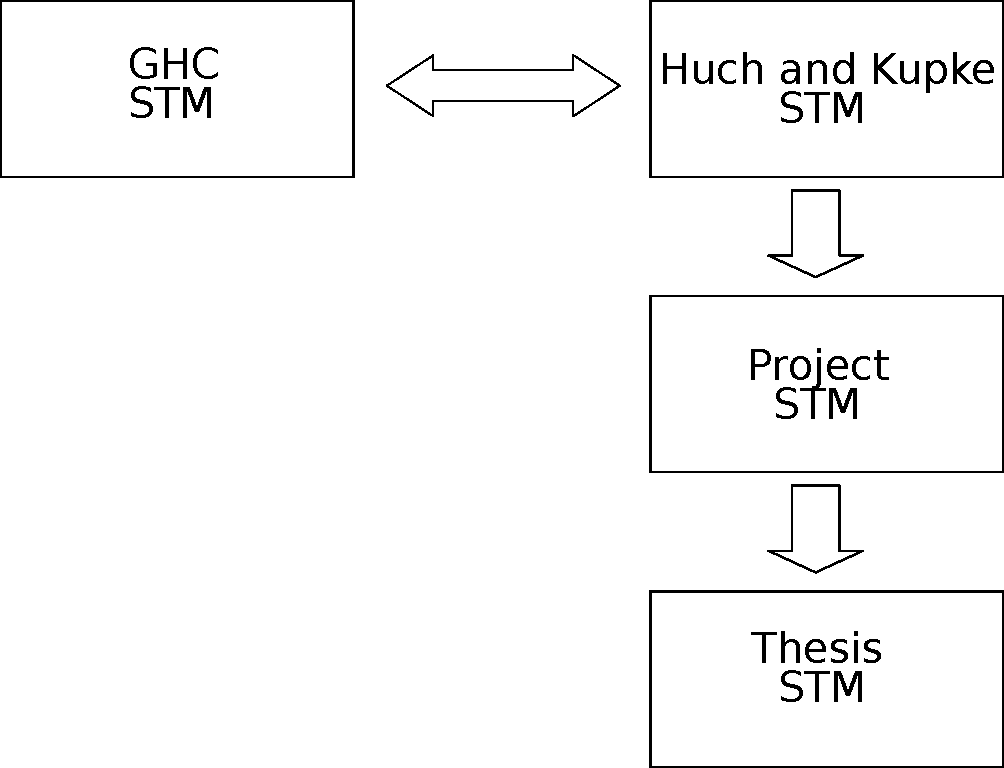
\includegraphics[scale=0.8]{Figures/implementations}
\decoRule
\caption[implementations]{The STM implementations for Haskell.}
\label{fig:implementations}
\end{figure}

\section{STM Types}
Before we head over to the implementation of the external interface of STM, we investigate the types
of STM that are used in this implementation starting with the STM type itself:
\begin{lstlisting}
 data STM a = STM (StmState -> IO (STMResult a))
\end{lstlisting}
In its core the STM data type is similar to a state monad. The IO type was initially needed to perform the reads 
in the computation phase. As we will see in the next section, in this implementation it is needed only to create new TVars
in the computation phase. \code{readTVar} and \code{writeTVar} do not need to process IO operations.
Thus an STM action takes a state and returns a result depending on this state. There are three possible 
results:
\begin{lstlisting}
 data StmResult a = Retry StmState
                  | InValid
                  | Success StmState (Maybe a)
\end{lstlisting}
The first constructor is used to indicate that \code{retry} occurred. This must be distinguished from 
\code{InValid}, since \code{orElse} and \code{atomically} react differently on these results. If 
\code{Retry} is returned, \code{atomically} validates and rolls back at an appropriate time; \code{orElse} 
starts the second transaction. This is the reason \code{Retry} is accompanied by the state.
The state holds the necessary information about the TVars that the transaction has read. This allows 
to validate and possibly suspend on particular TVars. \code{InValid} on the otherhand indicates
always that the transaction is not valid and thus must be restarted. 
The last constructor is the desired outcome of an action. If the transaction does not fail, it returns
\code{Success} and a state as well as the result. As before the state is needed for validation.
The result is wrapped with the \code{Maybe} type. The value \code{Nothing} never occurs. 
The reason for this wrapping is explained in Section \ref{sec:IFFun}. 

Before we examine the StmState, we need to take a look at the \code{TVar}
\begin{lstlisting}
 data TVar a = TVar (MVar (IORef a))
                    ID
                    (MVar [MVar ()])
                    (MVar ())
\end{lstlisting}
All TVars have a globally unique identifier called \code{ID}, which is immutable. The \code{MVar (IORef a)} 
holds the actual value of the TVar. The MVar is used to synchronize multiple transaction, if they intend to 
access the same TVar. The \code{IORef} is needed to enable a correct validation, which is explained in detail
in \ref{sec:IFFun}. \code{MVar [MVar ()]} is the queue of the MVar where transactions that wait on a change
enter their their personal \code{MVar ()}. Remember that this is needed to delay the rollback when \code{retry}
is evoked. The last part is an explicit lock for this TVar. There are currently two implementations as 
a result of this thesis. One of these implementations locks a TVar via 
the explicit lock and the other by taking the MVar that holds the value. The details are explained later. 

The computation phase does not allow any observable side effect and its only result is the \code{StmState} and 
a single value.
Hence, the core data structure is the \code{StmState} which holds all informations to commit a transaction:
\begin{lstlisting}
 data StmState = TST {writeSet   :: IntMap (Maybe (),
                                            Maybe (),
                                            MVar (IORef ())),
                      notifies   :: IO (),
                      readSet    :: ReadSet,
                      retryMVar  :: MVar (),
                      uEReads    :: [Maybe ()]}
\end{lstlisting}
The \code{writeSet} is similar to the log in the GHC implementation. Here it is an \code{IntMap} 
\footnote{This refers to the IntMap in the standart libraries of Haskell: \url{https://hackage.haskell.org/package/containers-0.5.8.1/docs/Data-IntMap-Strict.html}}. 
The keys are the IDs of the associated TVars. The elements contain the \code{expectedValue},
the \code{newValue}, and \code{actualMVar}. The \code{actualMVar} is the value holding MVar of the TVar and is needed in the commit
phase when the transaction sucessfully commits to publish its modifications. We already know the 
\code{expectedValue} and the \code{newValue} from \ref{sec:GHCImpl}, but their purpose is slighty 
different. The \code{Maybe} type indicates that the values also can be \code{Nothing}. This holds
only for the second entry. The first entry has the \code{Maybe} type for the same reason 
\code{Success} has it. The second entry on the other hand can become \code{Nothing}. This indicates
that the TVar was read but not written by the transaction. Note that there are two kinds of 
\textit{read}. The first is that a \code{readTVar} operation is porcessed in the computation phase
and the second that the current value of the TVar is read. In the original implementation these 
two occur always at the same time. In the new approach theses kinds of reads occur at different times.
For clearity, from here on I will use IO-reads when I refer to a read from the actual IORef to access
the current value of that TVar. Since Haskell does not provide a simple solution for inhomogeneous
containers, I decided to use the type \code{()} and cast all values via \code{unsafeCoerce} before
entering them to the \code{writeSet}. Whenever a value is taken from the \code{writeSet} it
is casted back to its original type by \code{unsafeCoerce}. The ID of the TVar ensures that 
the type it was casted from does not differ from the type it is casted to.

\code{nofifies} holds an IO action that is process when the transaction successfully commits.
This IO action notifies all transactions that are waiting on a TVar that is modified by the 
committing transaction.

\code{readSet} stores information about the IO-reads that where performed. The type \code{ReadSet}
is defined as follows\footnote{Notice the difference between 
\code{readSet} and \code{ReadSet}. \code{readSet} is the field of the \code{StmState} and 
\code{ReadSet} is the data type.}:
\begin{lstlisting}
 type ReadSet = IORef (InMap (IORef (), 
                              MVar (IORef ()), 
                              MVar [MVar ()]))
\end{lstlisting}
The need for the outermost IORef is explained later. This type is like the \code{writeSet} an 
\code{IntMap}. The keys are the IDs of the TVars. The entries consist of three parts. First,
the value (in form of the IORef) that was present when the IO-read was executed. Second, the 
MVar of the TVars that hold the value. Third, the queue of the associated TVar.
The exact ussage of this is explained in the next section.

\code{retryMVar} is a unique MVar for every transaction. This is the MVar that is entered into
the queues of the TVars when the transactions processes \code{retry}.

\code{uEReads}(unevaluated read) contains all unevaluated IO-read operations. This is essential to be able to 
process the IO-reads that where not evaluated in the computation phase. The \code{Maybe} type
is again used for the same reasons as it is in \code{StmResult}.

This concludes the overview on the data structures used and we can head over to see how these
data structures are used to implement the STM interface.





\section{Interface Functions}
\label{sec:IFFun}
Here we will inspect the implementation of every interface function. 

\subsubsection{newTVar}
\label{sec:newTVar}
This is the only function (besides \code{atomically}) that uses IO actions. A TVar consists of three MVars
and one ID. To ensure the uniqueness of the IDs the STM library defines \code{globalCount :: MVar Int}
and a function \code{getGlobalId :: IO Int} that takes the \code{globalCount}, increments it, writes it back 
and returns the old value. Due to the semantics of the MVar only one thread at a time can get an ID. 
No ID is assigned twice unless \code{globalCount} overflows. Because the chances that this happens 
are narrow, no countermeasures are performed to detect or avoid this problem. 

All MVars are created with \code{newMVar}. This means all MVars are initialized when the TVar is created.
The queue holds and emppty list the lock holds unit and the value hold an IORef with the passed value.
In the end the unchanged state as well as the new TVar is returned.

Lets take a look at the following example:
\begin{lstlisting}
transaction = do 
  tv <- newTVar 5
  a <- readTVar tv
  writeTVar tv (a + 1)
\end{lstlisting}
The first action of this transaction is the creation of a new TVar. This means a new IORef with 
the value \code{5} is created. After that three new \code{MVars} are created. The first contains the 
IORef, the second \code{[]} and the third \code{()}. With a the value gained from 
\code{getGlobalId} a new TVar is created. We assume the ID is \code{1} for now. 
The state on the other hand is not modified. Then the 
second action, \code{readTVar tv}, is processed.


\subsubsection{readTVar}
This function is the core of the new implementation. One part of \code{readTVar} is similar to the original 
Implementation. If the TVar is present in the \code{writeSet}, the \code{expectedValue} is returned (explained together with \code{writeTVar}).
The differences are in the other part of \code{readTVar}. Recall the type of \code{readTVar :: TVar a -> STM a}.
The result is an STM action. This means a function that takes a \code{StmState} and returns an \code{StmResult}. 
Unless the result is \code{InValid}, it contains a \code{StmState}. In other words, \code{readTVar} transforms
the state and returns the value of the TVar. To return the value of the TVar it would be needed to IO-read the
TVar. To avoid this the read is not executed directly. The function \code{buildVal} helps us to achieve this.

\code{buildVal} wraps
the value with \code{unsafePerformIO}. \code{unsafePerformIO} allows us to execute IO actions in pure
Haskell code. These IO actions are executen when the evaluation of the expression that they occur in 
is demanded. In this case the IO action consists of two parts. First, it IO-reads the 
current value of the TVar and returns it after wrapping in into \code{Just}. The wrapping with 
\code{Just} is explained when we examine the implementation of atomically. Second, entering the 
information to the \code{readSet} that are needed to validate. These are the ID of the TVar as 
key, the MVar of the TVar that holds the value, the value that the transaction saw when it IO-reads
the TVar, and the queue of that TVar. The value the transaction has seen in created by the first 
part of the \code{unsafePerformIO} action. The other information are the arguments of \code{buildVal}. After \code{buildVal}
created this wrapping, the expression is (from Haskells view) a normal expression, but the IO-read is
performed when the evaluation of the expression is demanded and not earlier; simultaneously is this 
evaluation logged in the \code{readSet}. Haskell demands the evaluation of values just to decide on
branch condition or to perform IO actions. IO actions are not allowed in the STM monad by the type
system. Thus the evaluation in the computation phase is only demanded when the control flow depends 
on it. 

Back to \code{readTVar}. \code{buildVal} is used to create the result. \code{readTVar} also modifies the 
the \code{StmState}. It adds the newly created value to \code{uEReads}. And it extends the writeSet.
At this point there is no entry for the TVar in the writeSet yet, otherwise this part of \code{readTVar}
would not be executed. A new entry is inserted. This entry contains the constructed value and 
the MVar that holds the value of the TVar. The \code{newValue} field of this entry is \code{Nothing}.
In the end the constructed value and the new state are returned in the \code{Success} constructor.

Reconsider the example givin in the previous section:
\begin{lstlisting}
transaction = do 
  tv <- newTVar 5
  a <- readTVar tv
  writeTVar tv (a + 1)
\end{lstlisting}
We explained already the first action. The first step of the second action is to lookup \code{tv}
in the \code{writeSet}. Since \code{tv} is not present in the \code{writeSet}, \code{buildVal} is
called to create the \code{unsafePerformIO} action. The result (called val in the 
following) is added to the \code{writeSet}. Thus the \code{writeSet} is no longer empty. It contains 
an entry for \code{tv}:
\begin{lstlisting}
 writeSet1 = {(1,(val, Nothing, mvar))}
\end{lstlisting}
\code{mvar} is the MVar of \code{tv} that holds the IORef with the value. The \code{1} is the
ID of \code{tv}. Aditionally is \code{val} 
added to \code{uEReads}. All other parts of the state are unchanged. Due to \code{<-}, \code{val} is 
bound to \code{a} in the end of the second action. 


\subsubsection{writeTVar}
This implementation is straight forward. Two modifications to the state are performed. One is
the modifications on \code{notifies}. A successful commit of the transaction would mean a 
modification to the TVar that \code{writeTVar} was called on. Thus this transaction 
possibly needs to notify waiting transactions. An IO action is created, that notifies
all transactions in the queue of the TVar. This IO action is sequenced by \code{>>} with 
\code{notifies} of the initial \code{StmState}. The resulting action then notifies all
TVars that are written by this transaction. This may lead to an action that notifies the 
same queue twice. This is a minor issue, becuase after the first notification the queue 
is emptied. To avoid this you would need to lookup the value in the writeSet, to see if 
it was already written and if so do not extend the \code{notifies} action. This look up
is most likely more expensive than a notification on an empty queue (this has not been 
investigated). 

The second modification that \code{writeTVar} performs is the modification of the \code{writeSet}.
After wrapping the value for type reasons with \code{Just}, it is entered in the \code{expectedValue} and \code{newValue} 
field of the associated entry in the \code{writeSet}. The last field of the entry is the MVar of
the TVar that holds the value. There is a reason to set both, the first and second field, to the
new value. If the second field is not \code{Nothing}, it indicates that this value is modified 
by the transaction and in the case the transaction sucessfully commits, the value in this field
is written. The first field of the entry is the field that \code{readTVar} returns if it finds
this entry. To avoid this doubled entry, the obvious choice were to use pattern matching to 
check whether the second value is \code{Nothing} and if not return that value. This does not
work in this implementation. The problem is that the pattern matching forces the evaluation.
By forcing the evaluation of an expression you may evaluate IO-reads and thus make TVars critical
that are not critical. This does not happen in the current implementation, because in every entry
of the \code{writeSet} the first field is always not \code{Nothing} and thus can be returned
without pattern matching on this value. 
In the end of \code{writeTVar}, the new state and \code{()} are returned.

For the example it means that the \code{writeSet} and \code{notifies} are modified by the third 
action. The \code{writeSet} looks like this after the third action\footnote{In fact \code{val} 
is of type \code{Maybe Int} and thus cannot be added to \code{1}. The bind operator on \code{STM}
unwraps the value, so we can use it as pure value. This means in the case, that the actual entries are
\code{Just (fromJust val + 1)}. For the sake of comprehensibility, we ignore this for now.}:
\begin{lstlisting}
 writeSet2 = {(1,(val + 1, val + 1, mvar))} 
\end{lstlisting}
In both, the first and the second field, \code{(val + 1)} is entered. \code{notifies} is 
initially \code{return ()}. After the \code{writeTVar} action it is:
\begin{lstlisting}
 notifies1 = do
    queue <- takeMVar waitQ
    mapM_ (flip tryPutMVar ()) queue
    putMVar []
    return ()
\end{lstlisting}
\code{waitQ} is the queue of \code{tv}. The notification is performed by trying to put \code{()}
to the MVars in the queue. It is important to use \code{tryPutMVar} instead of \code{putMVar}.
Otherwise the implementation contains a deadlock (imagine two transactions try to notify the same 
transaction at the same time). In the end the queue is emptied to avoid another transaction to 
notify the same transactions again. The final \code{return ()} is the initial value of 
\code{notifies}. The result of the three action in the example is:
\begin{lstlisting}
 Success state ()
\end{lstlisting}
\code{state} is a \code{StmState} that contains \code{notifies1}, \code{writeSet2} and the 
modified \code{uEReads}. The \code{readSet} and \code{retryMVar} are similar to the one 
in the initial state. This state is used in atomically to commit the changes.


\subsubsection{atomically}
This is the heart of every STM implementation in Haskell; it allows the user to execute STM 
actions in a transactional manner. Before \code{atomically} starts the computation phase, it
creates an initial state. This state basically holds no information and commit with this state
would result in no change at all. After the initial state is created, the computation phase starts. 
In this phase atomically does not do anything but pasing the initial state to the STM action.

After the \code{StmResult} is calculated, atomically starts the commit phase by interpreting
the result. There are three possible outcomes.
First, the result is \code{InValid}. If this occurs the computation phase is just restarted 
with the initial state\footnote{Actually the \code{readSet} needs to be discarded explicitly,
because it is an IORef and thus would not be empty by taking the initial state.}. 

Second, the result is \code{Retry newState}. This casues the transaction to lock the TVars in its 
\code{readSet} which can be accessed via \code{newState}. After the locks has been acquired, 
the \code{readSet} is validated. If it is not valid, the locks for the TVars are released and
the transaction is rolled back like it was done for \code{InValid}. If the transaction is 
valid, the transaction enters its \code{retryMVar} to the queue of the TVars it has read.
These queue are stored in the \code{readSet}. Then the transaction realeases the locks and 
executes a \code{takeMVar} on its \code{retryMVar}. This lets the transaction suspend until
another transaction notifies it. After the transaction was notified, it removes its 
\code{retryMVar} from the queue (if that has not already happend) and restarts.

Third, the result is \code{Success newState result}. This is the most interessting case, 
because it is the commit phase and thus leads not necessarily to a rollback, in contrast to 
the other two results. 
There are currently two different implementation as a result of this thesis which 
only differ in this part. The performance tests presented in Chapter \ref{Chapter4} do
not provide a clear result on which implementation is better in general. I will present
both implementation. When is it not clear which of the implementation we are talking about,
we will refer to the first implementation as STMLA (STM lock all) and the second STMWSL 
(STM write set lock). 

STMLA starts the commit phase by locking all TVars is has accessed. This implementation 
uses the explicit locks of the TVars. This information are 
stored in the \code{writeSet}, since \code{writeTVar} as well as \code{readTVar} create
entries for that are not part of the \code{writeSet}, but processed by either of these 
functions. When all locks are acquired, the transaction validates its \code{readSet}.
If this is not valid, the transaction is rolled back.
If it is valid, the transaction evaluates all expressions in \code{uEReads}. This is done
by the \code{seq} function, which forces the evaluation of its first argument and returns 
its second argument. As always in Haskell the expression is evaluated to WHNF\footnote{In 
case you do not know what \keyword{weak head normal form} is please refer to 
\url{https://wiki.haskell.org/Weak_head_normal_form}}. This is where the \code{Maybe} type 
comes in handy. \code{buildVal} created a \code{Maybe} value that was wrapped with an
\code{unsafePerformIO} action. If we force the evaluation of this expression, the 
IO-read is performed, but the underlying expression is not evaluated, because it is wrapped 
in the \code{Just} constructor. Without this constructor, we would evaluate the expression that 
is stored in the TVar. Imagine this expression is a complex computation. This means, we 
suffer a performance overhead because the computation is not yet needed (even worse if the
computation is not needed at all). 
Even worse we execute this in the commit phase, while we hold the locks for many TVars.
To maximize parallelism, we aim to minimize the time in the commit phase. Besides these
performance problems, there is a serious semantic problem. Everytime we force the 
evaluation of an expression that is not needed, we change the semantics of the program.
This may lead to exceptions or loops that would not occur normaly.
After the \code{uEReads} are evaluated, the actual writes are prepared. The writes are 
divided in two parts. First take the value from the MVar and second write the new value.
Preparing means all the value holding MVars of all TVars that are going to be written
are emptied. Then the \code{notifies} are processed. At last the new values are written
to the value holding MVars. This is needed to prevent a very nasty bug \footnote{For 
interessted readers is this bug explained in the appendix.}. 
The last step of the commit phase before returning the result is to realease the locks
that were taken at the start of the commit phase.

The second implementation (STMWSL) starts the commit phase by validating. As before, the 
transaction is rolled back if it is invalid. If it is valid, the remaining reads in 
\code{uERead} are evaluated. After all reads have been processed, the actual writes are
prepared. This means the TVars that are modified by the transaction are accessed and
their value holding MVar is emptied. At this point no other transaction is able to 
either read or write these TVars. In the first implementation the explicit locks 
were taken, which does not prevent other transactions from reading these TVars.
When the writes are prepared, the transaction is validated again. In contrast to 
the first validation, this validation is mandatory. It is possible that the current
values of the TVars have changed after the reads were processed and before the 
writes were prepared (and by this the TVars locked). The first validation is
added to avoids the problem that the transaction acquires the locks, although it 
is invalid. The costs for locking are much higher than the costs for validation.
If the transaction is invalid after the reads are processed and the transcation
acquired the locks, it is rolled back. If it is valid the it is similar to
the first implementation (STMLA). At first the \code{notifies} are processed
and then the writes are processed. At last the result is returned. Note that
it is not necessary to unlock the TVars explicitly, because only the value 
holding MVars of the TVars serve as a lock in STMWSL. By filling these MVars
the associated TVar is unlocked. 

Both implementation have their own benefits. STMLA does never roll back,
when the transaction does not branch at all. If two transactions read the
same TVar they cannot commit at the same time in STMLA. In STMWSL it is
possible that two transaction, that read the same TVar, commit simultaneously
(if non of them also writes this TVar). It is also possible
that a rollback occurs, even if the transaction does not branch. The 
problem is that the remaining reads are evaluated in an unlocked context.
This means that other transactions can modify these values after they were 
read and thus invalidate the reading transaction. It would be better, if the
transaction process the \code{uEReads} after it has locked the TVars. This is 
currently not possible. As we will discuss in detail in the next section, when 
we only lock the modified TVars, it is essential that no other transaction 
reads them while we hold the locks. Otherwise the ACI properties cannot be 
guaranteed. If we take the value holding MVars it prevents other transactions
from reading the associated TVars. Unfortunately, this also prevents us from 
reading the TVars. That is why we need to process \code{uEReads} before we 
acquire the locks for the TVars. The clever reader may have noticed that 
we get the values of the TVars when we prepare the writes, because we execute
\code{takeMVar} on the value holding MVars. To use these information would 
require the \code{unsafePerformIO} actions produced by \code{buildVal} to 
behave diffrently when it is executed in the computation phase and in the 
commit phase. Nevertheless, this topic remains for future work and is discussed 
in Chapter \ref{Chapter5}.

A solution that combines STMLA and STMWSL would be better\footnote{This could 
not be proved, because no such implementation is present currently.}.
A combined solution locks the TVars that the transaction has modified in a 
manner that no \textbf{other} transaction can read them. The transaction itself
is still able to read the locked TVars. Then the transaction is validated. 
If it is valid, the remaining reads are processed and the transaction publishes
its modifications. At last the transaction returns the result, after unlocking
the TVars.

If we execute \code{transaction} introduced in Section \ref{sec:newTVar} with 
\code{atomically} (of STMLA), the computation phase produces the previously mentioned state.
This \code{writeSet} in this state contains a single entry. The entry for the
newly created TVar. The commit phase starts by validating the \code{readSet}. 
Since the \code{readSet} is empty, the validation succeeds and the transaction
acquires the lock for \code{tv}. After the lock is acquired, the transaction 
evaluates \code{uEReads}. \code{uEReads} contains one value, namely \code{val},
the {unsafePerformIO} action that reads \code{tv}. The evaluation of this value 
has (thanks to sharing) an effeect on the \code{writeSet} as well:
\begin{lstlisting}
 writeSet = {(1,(Just (5 + 1), Just (5 + 1), mvar))} 
\end{lstlisting}
The next step in to prepare the writes. This means \code{mvar} is emptied via 
\code{takeMVar}. Before it is filled again, \code{notifies} is executed. \code{notifies}
does nothing because the \code{waitQ} of \code{tv} is empty. Finally the expression (\code{5 + 1})
written to \code{mvar}. Note that the expression itself is not evaluated. The last step
before returning \code{()} is to release the lock for \code{tv}.

\subsubsection{>>=}
The monadic bind operator, \code{>>=}, is an important part of the interface, because it allow us 
to use the do-natation. The aim of this thesis is to provide an alternative STM 
implementation for Haskell without altering the semantics or interface. One of 
the most comfortable things about is the way we use it. Thus it is important to 
retain this feature. \code{>>= :: STM a -> (a -> STM b) -> STM b} allows us to 
extract the result of an \code{STM} action from the STM context and use it to create 
a new STM action. Additionally it is used to translate \code{<-} of the do-notation.
The implementation is straight forward, but for the sake of completeness presented
nonetheless. The result is a STM action, meaning that it is a function that takes 
a \code{StmState} and its result is a \code{StmResult}. Thus the function basically
has three arguments. The \code{STM} action, the function of type \code{a -> STM b},
and the \code{StmState}. These arguments are called \keyword{passed action/function/state}
in the following. 

The resulting function first applies the passed state to the passed action. 
If the result is \code{InValid}, it just returns \code{InValid}. If it is
\code{Retry newState} it returns \code{Retry newState}. 

Note that it is important to 
pass the \code{newState} created by the action, because it contains information that
are needed to wait before rolling back. 

If the result of the action is 
\code{Success newState res}, the function first needs to unwrap \code{res}; it is wrapped with 
the \code{Just} constructor. This is done by the partial function \code{fromJust}. The
implementation ensure that \code{Nothing} can never occur and thus the call to 
\code{fromJust} is safe. After the value is extracted, it is applied to the passed 
function. This application results in a \code{STM} action. To gain \code{StmResult} as 
the result of the function the \code{newState} is applied to the action.
Thanks to the laziness of Haskell the call to \code{fromJust} is not evaluated 
immediately. This is the key of this implementation, since we avoid the evaluation of 
the IO-read by this. If \code{fromJust} would be evaluated when the bind operator is evaluated,
a action like \code{a <- readTVar t1} would not differ from the original implementation,
because the \code{unsafePerformIO} action would be executed immediately. 
Since we use a \code{case} expression to branch on the different \code{StmResult}s, we 
could also extract the value from the \code{Maybe} type  via pattern matching instead 
of \code{fromJust}. This would also lead to the evaluation of the value and 
make the wrapping performed by \code{buildVal} futile.

\subsubsection{retry and orElse}
The implementation of \code{retry} and \code{orElse} are very simple. 
\code{retry} is a STM action. The passed state is wrapped with the \code{Retry} constructor.
That is all \code{retry} does. 

\code{orElse} executes the first acion with the passed state and if the result is not 
\code{Retry newState} it just returns this result. If it is \code{Retry newState},
the second action is executed with the passed state (not the \code{newState}) to discard the 
writes executed by the first action. Since the \code{readSet} is an \code{IORef}, 
we do not lose the information on the TVars that was read. 



\section{Notes on the Implementation}
Some details of the implementation remained unexplained until here. These details are highlighted
in this section.

\subsubsection{Deadlock Avoidance}
One Motivation for STM is the deadlock freedom. We have seen in Section \ref{STMInterface} that acquiring 
multiple locks always includes the danger of deadlocks if multiple threads work concurrently. 
There are two concepts to avoid deadlocks for such settings. The setting is that multiple threads
try to acquire and arbitrary number of shared locks. The first avoidance strategy is, if thread tries to 
acquire a lock that is not available, the thread releases all locks and tries to acquire all locks again.
This is continued until the thread can acquire all desired locks. The other avoidance strategy is to 
acquire the locks in a global order. STMLA as well as STMWSL use the latter. The TVars that need to be 
locked are stored within \code{IntMap}s. If a transaction trys to lock these TVars, the transaction converts 
the \code{IntMap} to a list and process it. Since the conversion from an \code{IntMap} constructs an ordered 
list, the transactions always locks in a global order. The TVars are ordered by their IDs.


\subsection{STMWSL}
The double validation of STMWSL seems to be an unnecessary overhead. However, the original implementation 
also uses this scheme, which was proposed by Fraser \parencite[Page 42]{lockfreedom}. The high costs for locking the TVars
are the reason. This locking itself is not particular expensive, but it hinders parallelism.
Everytime a TVar is locked no other transaction is able to read, lock, or validate this TVar. Additionally if 
a transaction tries to access a locked TVar, it is suspended and a context switch follows. Context switches in Haskell 
are not as expensive as context switches of OS threads, but it schould not be neglected, especially when dealing
with a large number of threads. Validation is a operation, which needs two memory access per entry in the log.
One memory access is the access to the log entry to look up the expected value and the other memory access is
the access to the actual TVar\footnote{The log entry needs to be accessed two times. First to get the expected
value and second to get the next entry, because the log is a dynamic structure and thus needs a pointer
to the next entry comparable to a list. Nevertheless the entry itself is (most likely) in one block in the memory.
This is why I consider one memory access to be enough for the entry.}. This is reasonable considering that the 
log only consists of TVars that are needed to determine the control flow. So validation is significant faster
than locking. 


